\section{Standar latex dan git}

\begin{enumerate}
\item sebelum melakukan langkah pull reques alangkah baik anda mempelajari materi git di github.com/bukuinformatika/git (buka file git.pdf)
\item buka github awangga/ppji (cari ppji.pdf untuk melihat penulisan standar latex)
\item buka github.com/bukuinformatika/keleketek (untuk mempelajari materi dasar latex)
\end{enumerate}

 langkah-langkah Pull request menggunakan GIT BASH:
\begin{enumerate}
\item git pull origin master
\item git pull upstream master
\item git push origin master
\item edit file yang akan di pull reques
\item setelah anda selesai edit/tambah file comflile dulu di main.tex agar anda tahu pekerjaan yang anda lakukan tidak bermasalah.
\item git status
\item git add 'namafile\_sesui\_setatus'
\item git staus 
\item commit -m 'melakukan apa yang anda edit'
\item git status
\item git pull upstream master
\item git push origin master
\end{enumerate}

Buka repositori anda untuk new pull request:
\begin{enumerate}
\item Klik New Pull request
\item Klik tombol hijau seperti pada gambar lihat tanda yang diberi kotak warna merah \ref{labelgambar1} 
		\begin{figure}[htbp]
		\centering
		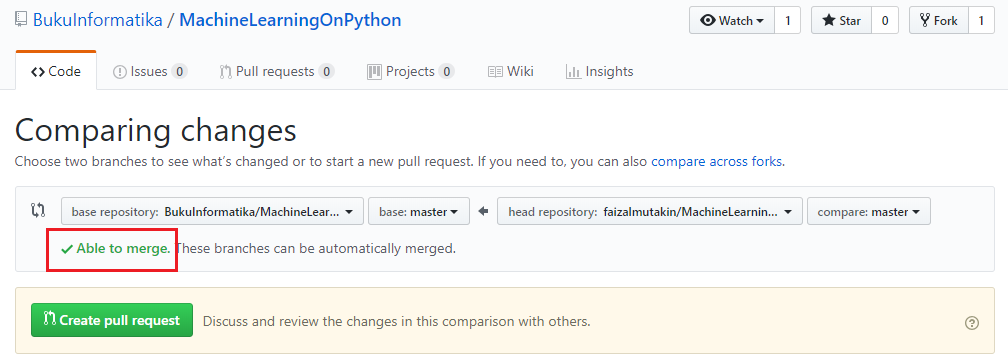
\includegraphics[width=1\textwidth]{figures/1.PNG}
		\caption{Gambar new pull requesh}
		\label{labelgambar1}
		\end{figure}	 
\end{enumerate}